\documentclass[a4paper,11pt]{amsart}

\usepackage{gensymb}

\usepackage{tikz}
\usetikzlibrary{arrows.meta}
\usepackage{caption}

\usepackage{times}
\usepackage[top=27mm, left=23mm, bottom=23mm, right=23mm]{geometry}
\usepackage{amsfonts, amssymb, amsgen, amsthm, amscd, amsmath}
\usepackage{mathtools}
\mathtoolsset{showonlyrefs=true}

\usepackage{bm}
%\usepackage{mathpazo}
\usepackage{domitian}
\usepackage[T1]{fontenc}
\let\oldstylenums\oldstyle

\usepackage{enumerate}
\usepackage{color}
\usepackage[all]{xy}

\newtheorem{theorem}{Theorem}[section]
\newtheorem{proposition}[theorem]{Proposition}
\newtheorem{lemma}[theorem]{Lemma}
\newtheorem{corollary}[theorem]{Corollary}
\newtheorem{claim}[theorem]{Claim}
\theoremstyle{definition}
\newtheorem{remark}[theorem]{Remark}
\newtheorem{example}[theorem]{Example}
\newtheorem{definition}[theorem]{Definition}

\newcommand{\outimes}[2]{\overset{#1}{\underset{#2}{\otimes}}}
\newcommand{\C}[1]{\mathcal{#1}}
\newcommand{\B}[1]{\mathbb{#1}}
\newcommand{\G}[1]{\mathfrak{#1}}
\newcommand{\rmod}[1]{\text{{\bf Mod}-}{#1}}

\newcommand{\Span}{\text{\rm Span}}
\newcommand{\Tor}{\text{\rm Tor}}
\newcommand{\Ind}{\text{\rm Ind}}
\newcommand{\Res}{\text{\rm Res}}
\newcommand{\Ext}{\text{\rm Ext}}
\newcommand{\Hom}{\text{\rm Hom}}
\newcommand{\CoInd}{\text{\rm CoInd}}
\newcommand{\Simp}{{\Delta}}
\newcommand{\Diff}{{\Omega}}
\newcommand{\xla}[1]{\xleftarrow{#1}}
\newcommand{\colim}{\text{colim}}
\renewcommand{\baselinestretch}{1.15}

\setlength{\parskip}{1.2mm}
\setlength{\parindent}{0mm}

\title{Electromagnetism Assignment For The Seventh Time}

\author{Haixuan Lin - 23307110267}
\email{23307110267@m.fudan.edu.cn}


\address{Fudan University, Physics Department, China}

\begin{document}
	
	\begin{abstract}
		Here is the electromagnetism assignment for the seventh time which is for the course given by professor Weitao Liu. In order to practise the expertise in scientific film of physics, students need to practise using \LaTeX to composing their own work, even if this is only a ordinary homework.
	\end{abstract}
	
	\maketitle
	\section*{Main Text}
	
	\subsection*{6-21}
	
	We need to calculate the change in the electric field energy across space, and according to the conservation of energy, this is equal to the work done by the external force.
	
	\begin{align}
		\Delta W_e&=\int_{R_1}^{R_2}{\left( \frac{1}{2}\boldsymbol{D}\cdot \boldsymbol{E}-\frac{1}{2}\varepsilon _0\boldsymbol{E}^2 \right) \cdot 4\pi r^2\mathrm{d}r}
		\\\\
		&=\int_{R_1}^{R_2}{\frac{1}{2}\varepsilon _0\boldsymbol{E}^2\left( \varepsilon _r-1 \right) \cdot 4\pi r^2\mathrm{d}r}
		\\\\
		&=\int_{R_1}^{R_2}{\frac{1}{2}\varepsilon _0\frac{Q^2}{4\pi \varepsilon _0\varepsilon _rr^4}\left( \varepsilon _r-1 \right) \cdot 4\pi r^2\mathrm{d}r}
		\\\\
		&=\frac{Q^2\left( \varepsilon _r-1 \right)}{8\pi \varepsilon _0\varepsilon _r}\left( \frac{1}{R_1}-\frac{1}{R_2} \right) 
	\end{align}
	
	\subsection*{7-1}
	
	For a uniformly charged rigid body, its contribution to the magnetic moment is studied by taking its upper microelement.
	
	\begin{align}
		\mathrm{d}m_{es}&=\frac{\mathrm{d}Q}{T}\pi r^2=\frac{\omega}{2\pi}\pi r^2\mathrm{d}Q=\frac{\omega}{2\pi}\frac{\rho _e}{\rho}\pi r^2\mathrm{d}m=\frac{\omega}{2\pi}\frac{Q}{m}\pi r^2\mathrm{d}m
		\\
		&=\frac{Q}{2m}\cdot r^2\mathrm{d}m\cdot \omega =\frac{Q}{2m}\cdot \mathrm{d}J\cdot \omega 
		\\
		m_{es}&=\frac{Q}{2m}J\omega =\frac{Q}{2m}L_s
	\end{align}
	
	This is different from what quantum mechanics tells us, which is $\displaystyle m_{es}=\frac{Q}{m}L_s$.
	
	\subsection*{7-2}
	
	The Lorente force give the contribute:
	
	$$
	qv'B+m\frac{v'^2}{r}=m\dfrac{v^2}{r}
	$$
	
	Base on the opinion that $r$ is a constant. So
	
	$$
	\Delta m_{el}=\dfrac{1}{2}q\Delta vr=3.94\times10^{-29}\,\mathrm{A\cdot m^2}
	$$
	
	$$
	\dfrac{\Delta m_{el}}{m_{el}}=4.2\times10^{-6}
	$$
	
	\subsection*{7-7}
	
	\subsubsection*{(1)}
	
	According to Ohm's law in differential form
	
	$$
	J=\frac{I}{\pi R^2}=\gamma E
	$$
	
	So $\displaystyle E=\frac{I}{\pi R^2\gamma}.$
	
	According to Ampere's loop theorem modified by Maxwell
	
	$$
	\oint{\boldsymbol{H}\cdot \mathrm{d}\boldsymbol{l}}=\oint{\frac{\boldsymbol{B}}{\mu _0\mu _r}\cdot \mathrm{d}\boldsymbol{l}=\frac{B}{\mu _0\mu _r}\cdot 2\pi r=\sum{I_c=I\frac{r^2}{R^2}}}
	$$
	
	We have $\displaystyle B=\frac{\mu _0\mu _rI}{2\pi R^2}r$.
	
	
	\subsubsection*{(2)}
		
	According to the definition of the magnetization vector
	
	$$
	\boldsymbol{M}=\frac{1}{\mu _0}\boldsymbol{B}-\boldsymbol{H}=\dfrac{1}{\mu_0}\left( 1-\dfrac{1}{\mu_r} \right)\bm{B} = \dfrac{1}{\mu_0}\left( 1-\dfrac{1}{\mu_r} \right)\frac{\mu _0\mu _rI}{2\pi R^2}r\bm{\hat{z}}
	$$
	
	According to vector $\bm{M}$ we can calculate magnetizing current
	
	\begin{align}
		\begin{aligned}
			\bm{j}_{M}^{\prime} &= \nabla \times \boldsymbol{M} = \frac{1}{\mu _0}\left( 1-\frac{1}{\mu _r} \right) \frac{\mu _0\mu _r I}{2\pi R^2}\cdot \frac{1}{r}\left| \begin{matrix}
				\hat{\boldsymbol{r}} & r\hat{\boldsymbol{\theta}} & \hat{\boldsymbol{z}} \vphantom{\dfrac{1}{1}} \\
				\dfrac{\partial}{\partial r} & \dfrac{\partial}{\partial \theta} & \dfrac{\partial}{\partial z} \\
				0 & 0 & r \vphantom{\dfrac{1}{1}} \\
			\end{matrix} \right| = -\frac{\left( \mu _r-1 \right) I}{2\pi R^2}\bm{\hat{\theta}} \\
			\boldsymbol{i}_{M}^{\prime} &= \boldsymbol{M}\times \hat{\boldsymbol{n}} = M\hat{\boldsymbol{\theta}} = \frac{\left( \mu _r-1 \right) I}{2\pi R}\hat{\boldsymbol{\theta}}
		\end{aligned}
	\end{align}
	
	The direction is about the picture below:
	
	\begin{minipage}{1.0\textwidth}
		\centering
		\tikzset{every picture/.style={line width=0.75pt}} %set default line width to 0.75pt  
		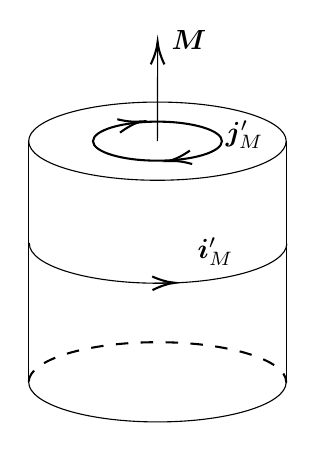
\begin{tikzpicture}[x=0.75pt,y=0.75pt,yscale=-1,xscale=1]
			%uncomment if require: \path (0,300); %set diagram left start at 0, and has height of 300
			
			%Shape: Ellipse [id:dp958487281710054] 
			\draw   (77.67,65.11) .. controls (77.67,54.71) and (105.44,46.27) .. (139.7,46.27) .. controls (173.96,46.27) and (201.73,54.71) .. (201.73,65.11) .. controls (201.73,75.51) and (173.96,83.95) .. (139.7,83.95) .. controls (105.44,83.95) and (77.67,75.51) .. (77.67,65.11) -- cycle ;
			%Straight Lines [id:da5923172725420689] 
			\draw    (77.67,65.11) -- (77.67,181.45) ;
			%Straight Lines [id:da9323842681079457] 
			\draw    (201.73,65.11) -- (201.73,181.45) ;
			%Shape: Arc [id:dp7282849048260578] 
			\draw  [draw opacity=0] (201.73,181.43) .. controls (201.37,191.92) and (173.74,200.38) .. (139.7,200.38) .. controls (105.44,200.38) and (77.67,191.81) .. (77.67,181.22) .. controls (77.67,181.13) and (77.67,181.03) .. (77.68,180.93) -- (139.7,181.22) -- cycle ; \draw   (201.73,181.43) .. controls (201.37,191.92) and (173.74,200.38) .. (139.7,200.38) .. controls (105.44,200.38) and (77.67,191.81) .. (77.67,181.22) .. controls (77.67,181.13) and (77.67,181.03) .. (77.68,180.93) ;  
			%Shape: Arc [id:dp31507321145597245] 
			\draw  [draw opacity=0][dash pattern={on 4.5pt off 4.5pt}][line width=0.75]  (77.68,180.92) .. controls (78.04,170.44) and (105.67,161.97) .. (139.71,161.97) .. controls (173.97,161.97) and (201.74,170.55) .. (201.74,181.13) .. controls (201.74,181.23) and (201.74,181.33) .. (201.73,181.42) -- (139.71,181.13) -- cycle ; \draw  [dash pattern={on 4.5pt off 4.5pt}][line width=0.75]  (77.68,180.92) .. controls (78.04,170.44) and (105.67,161.97) .. (139.71,161.97) .. controls (173.97,161.97) and (201.74,170.55) .. (201.74,181.13) .. controls (201.74,181.23) and (201.74,181.33) .. (201.73,181.42) ;  
			%Straight Lines [id:da703025827800001] 
			\draw    (139.7,65.11) -- (139.77,25.17) -- (139.78,19.18) ;
			\draw [shift={(139.78,17.18)}, rotate = 90.1] [color={rgb, 255:red, 0; green, 0; blue, 0 }  ][line width=0.75]    (10.93,-3.29) .. controls (6.95,-1.4) and (3.31,-0.3) .. (0,0) .. controls (3.31,0.3) and (6.95,1.4) .. (10.93,3.29)   ;
			%Shape: Ellipse [id:dp8915554251324997] 
			\draw  [line width=0.75]  (108.64,65.11) .. controls (108.64,59.92) and (122.55,55.7) .. (139.7,55.7) .. controls (156.85,55.7) and (170.76,59.92) .. (170.76,65.11) .. controls (170.76,70.3) and (156.85,74.51) .. (139.7,74.51) .. controls (122.55,74.51) and (108.64,70.3) .. (108.64,65.11) -- cycle ;
			%Straight Lines [id:da61095448092952] 
			\draw    (148.66,74.1) -- (147.08,74.37) ;
			\draw [shift={(145.11,74.7)}, rotate = 350.46] [color={rgb, 255:red, 0; green, 0; blue, 0 }  ][line width=0.75]    (10.93,-3.29) .. controls (6.95,-1.4) and (3.31,-0.3) .. (0,0) .. controls (3.31,0.3) and (6.95,1.4) .. (10.93,3.29)   ;
			%Straight Lines [id:da835466478950259] 
			\draw    (124.36,57.1) -- (129.77,56) ;
			\draw [shift={(131.73,55.61)}, rotate = 168.56] [color={rgb, 255:red, 0; green, 0; blue, 0 }  ][line width=0.75]    (10.93,-3.29) .. controls (6.95,-1.4) and (3.31,-0.3) .. (0,0) .. controls (3.31,0.3) and (6.95,1.4) .. (10.93,3.29)   ;
			%Shape: Arc [id:dp9003535146279609] 
			\draw  [draw opacity=0] (202.03,114.61) .. controls (201.67,125.09) and (174.03,133.56) .. (140,133.56) .. controls (105.74,133.56) and (77.97,124.98) .. (77.97,114.4) .. controls (77.97,114.3) and (77.97,114.21) .. (77.97,114.11) -- (140,114.4) -- cycle ; \draw   (202.03,114.61) .. controls (201.67,125.09) and (174.03,133.56) .. (140,133.56) .. controls (105.74,133.56) and (77.97,124.98) .. (77.97,114.4) .. controls (77.97,114.3) and (77.97,114.21) .. (77.97,114.11) ;  
			%Straight Lines [id:da6061811179257774] 
			\draw    (138.3,133.56) -- (146.16,133.38) ;
			\draw [shift={(148.16,133.34)}, rotate = 178.69] [color={rgb, 255:red, 0; green, 0; blue, 0 }  ][line width=0.75]    (10.93,-3.29) .. controls (6.95,-1.4) and (3.31,-0.3) .. (0,0) .. controls (3.31,0.3) and (6.95,1.4) .. (10.93,3.29)   ;
			
			% Text Node
			\draw (145.25,10.7) node [anchor=north west][inner sep=0.75pt]    {$\boldsymbol{M}$};
			% Text Node
			\draw (171.41,53.85) node [anchor=north west][inner sep=0.75pt]    {$\boldsymbol{j}_{M}^{\prime }$};
			% Text Node
			\draw (157.78,110.19) node [anchor=north west][inner sep=0.75pt]    {$\boldsymbol{i}_{M}^{\prime }$};
			
			
		\end{tikzpicture}
		
	\end{minipage}

	\subsection*{7-9}
	
	The graph is as follow:
	% TODO: \usepackage{graphicx} required
	\begin{figure}[h]
		\centering
		\includegraphics[width=1\linewidth]{7-9}
		\caption*{Graph for 7-9}
		\label{fig:7-9}
	\end{figure}
	
	\subsection*{7-14}
	
	\subsubsection*{(1)}
	
	Let the Angle between the magnetic induction vector and the normal line in the medium be $\beta$ according to the magnetic induction refraction formula:
	
	$$
	\frac{\mu _r}{1}=\frac{\tan \beta}{\tan \theta}
	$$
	
	And the normal component of the magnetic induction vector is always continuous:
	
	$$
	B^{\prime}\cos \beta =B\cos \theta 
	$$
	
	As a result:
	
	$$
	\beta =\mathrm{arc}\tan \mu _r\tan \theta 
	$$
	
	$$
	B^{\prime}=\frac{\cos \theta}{\cos  \mathrm{arc}\tan \mu _r\tan \theta}B=\sqrt{\mu _{r}^{2}\sin ^2\theta +\cos ^2\theta}B
	$$
	
	\subsubsection*{(2)}
	
	According to the definition of magnetization:
	
	$$
	M_{\tau}^{\prime}=\frac{B^{\prime}\sin \beta}{\mu _0}\left( 1-\frac{1}{\mu _r} \right) 
	$$
	
	With it property:
	
	$$
	i_{M}^{\prime}=M_{\tau}^{\prime}=\frac{1}{\mu _0}\left( \mu _r-1 \right) B\sin \theta 
	$$
	
	\subsection*{8-2}
	
	So
	
	$$
	X_C=X_L
	$$
	
	$$
	\dfrac{1}{\omega C}=\omega L
	$$
	
	As a result $\omega=\dfrac{1}{\sqrt{LC}}.$
	
	$$
	f=2\pi\omega=1678\,\mathrm{Hz}
	$$
	
	$$
	X_C=X_L=31.6\,\mathrm{\Omega}
	$$
	
	\subsection*{Left-Handed Metamateria}
	
	% TODO: \usepackage{graphicx} required
	\begin{figure}[h]
		\centering
		\includegraphics[width=0.5\linewidth]{handed}
		\caption*{Left-Handed Metamateria}
		\label{fig:handed}
	\end{figure}
	
	\subsubsection*{Proof the $\gamma<0$}
	
	By the refraction formula of electric field intensity, we can assert that the $\gamma<0.$
	
	$$
	\frac{\tan  \mathrm{i}}{\tan \gamma}=\frac{1}{\varepsilon _r}
	$$
	
	\subsubsection*{Proof $\bm{S'}//-\bm{k}$}
	
	In the material we have
	
	$$
	\bm{S'}=\bm{E}\times \bm{H}=\bm{E}\times\left( \dfrac{1}{\mu_0\mu_{r}}\bm{B}\right) =\bm{E}\times\left( \dfrac{1}{\mu_0\mu_{r}\omega}\bm{k}\times \bm{E}\right)=\frac{1}{\mu _0\mu _r\omega}E^2\boldsymbol{k}
	$$
	
\end{document}

